\documentclass[final]{anthology-ch}

\usepackage{booktabs}
\usepackage{graphicx}

\usepackage{csquotes}\MakeOuterQuote{"}
\usepackage{todonotes,soul,comment}
\usepackage{float}

\ExecuteBibliographyOptions{maxnames=50}
\sloppy

\title{Classifying Medieval Manuscripts by Pen and Support}

\author[*]{Sharva Gogawale}[orcid= 0009-0000-5230-5197]

\author[*]{Omer Ventura}[orcid=
]

\author[*]{Daria {Vasyutinsky-Shapira}}[orcid=0000-0002-4257-7882]

\author[*]{Berat {Kurar-Barakat}}[
orcid=0000-0002-7240-7286]

\author[*]{Gal Grudka}[
orcid=
]

\author[*]{Mohammad Suliman}[
orcid=
]

\author[*]{Iddo Hakim}[
orcid=
]

\author[*]{Nachum Dershowitz}[
orcid=
]

\affiliation{*}{School of Computer Science and AI, Tel Aviv University, Ramat Aviv, Israel}

\keywords{manuscripts, pen, support, substrate, paper, parchment, quill, calamus, classifiers, CNN}

\pubyear{2025}
\pubvolume{3}
\pagestart{1349}
\pageend{1359}
\conferencename{Computational Humanities Research 2025}
\conferenceeditors{Taylor Arnold, Margherita Fantoli, and Ruben Ros}
\doi{10.63744/tL5xGcaScd42}
\paperorder{82}

\addbibresource{bibliography.bib}

\begin{document}

\maketitle

\begin{abstract}
We present a machine-learning approach for classifying medieval Hebrew manuscripts by two key material attributes: writing support (whether the substrate is paper or parchment) and writing implement (quill pen vs.\@ reed calamus).
Our work contributes to the emerging field of computational codicology, offering tools to aid paleographers in the large-scale analysis of digitized manuscripts.
Our datasets---derived from existing digitized repositories---

have been carefully annotated and balanced to capture the range of material and stylistic variation.
For both classification tasks, we employ convolutional neural networks tailored to their respective challenges: identifying broad substrate textures and capturing fine-grained stroke morphology.
The support classifier achieved an accuracy of 91\% and demonstrated reliable performance even on visually ambiguous examples.
Likewise, the implement classifier was 91.5\% accurate.
These findings show that computational analysis can aid and, in some cases, surpass manual paleographic methods in analyzing historical manuscripts.
This work highlights the potential of computational tools to assist scholars in large-scale analysis of digitized corpora, aiding manuscript dating, provenance research, and the study of scribal practices.
\end{abstract}

\section{Introduction}

The National Library of Israel, as part of its Ktiv project,
\footnote{\url{https://www.nli.org.il/en/discover/manuscripts/hebrew-manuscripts}}
has been digitizing most of the surviving approximately one hundred thousand Hebrew-character manuscripts that sit in libraries and collections in Europe and elsewhere~\cite{NLIKtiv}.
About ten million images are expected with the completion of the project in the near future.
Unfortunately, precious few of the manuscripts include the date or location of its writing.

For centuries, parchment served as the primary material for a wide array of media, ranging from sumptuously decorated religious texts to practical everyday documents.
This writing support

remains an invaluable source of historical, artistic, cultural, and even biological information~\cite{biocodical}.
The use of skins---those of calves, sheep and goats---for the writing of scrolls was standard among Jews already at around the time of the canonization of the Hebrew Bible two millennia ago.
The type of processing of the skin depended on the type of manuscript.
Most of the Dead Sea
scrolls are written on \textit{gevil}, a hide processed for writing on one side only, as required by the scroll format.
Medieval manuscripts, which often take the form of a codex (bound book form), were made from parchment, with the leather skin processed for writing on both sides.
The even earlier type of writing support, papyrus---made of leaves of the papyrus sedge, was still used for many Judaean desert documents in classical times, but, by the Middle Ages, parchment gradually became the standard writing support due to its flexibility, which made it better suited to the codex structure while lending itself to writing on both sides of a leaf.

Thus, in the Middle Ages, Hebrew manuscripts were written on two kinds of substrates only: parchment made from skins of sheep and cattle, or paper, produced from linen rags, or sometimes---in the Mediterranean---from cotton.
The use of parchment preceded the use of paper by hundreds of years, and in the Islamic lands the transition from the expensive parchment to cheap paper happened much earlier than in Christian countries.

\begin{figure}[t]
\centering
\begin{tabular}{c c c}
& Calamus & Quill \\
\raisebox{1.5cm}{\rotatebox{90}{Parchment}}&
\includegraphics[trim=500 1450 900 255,clip,width=0.38\linewidth]{figures/calamus on parchment.jpg} &
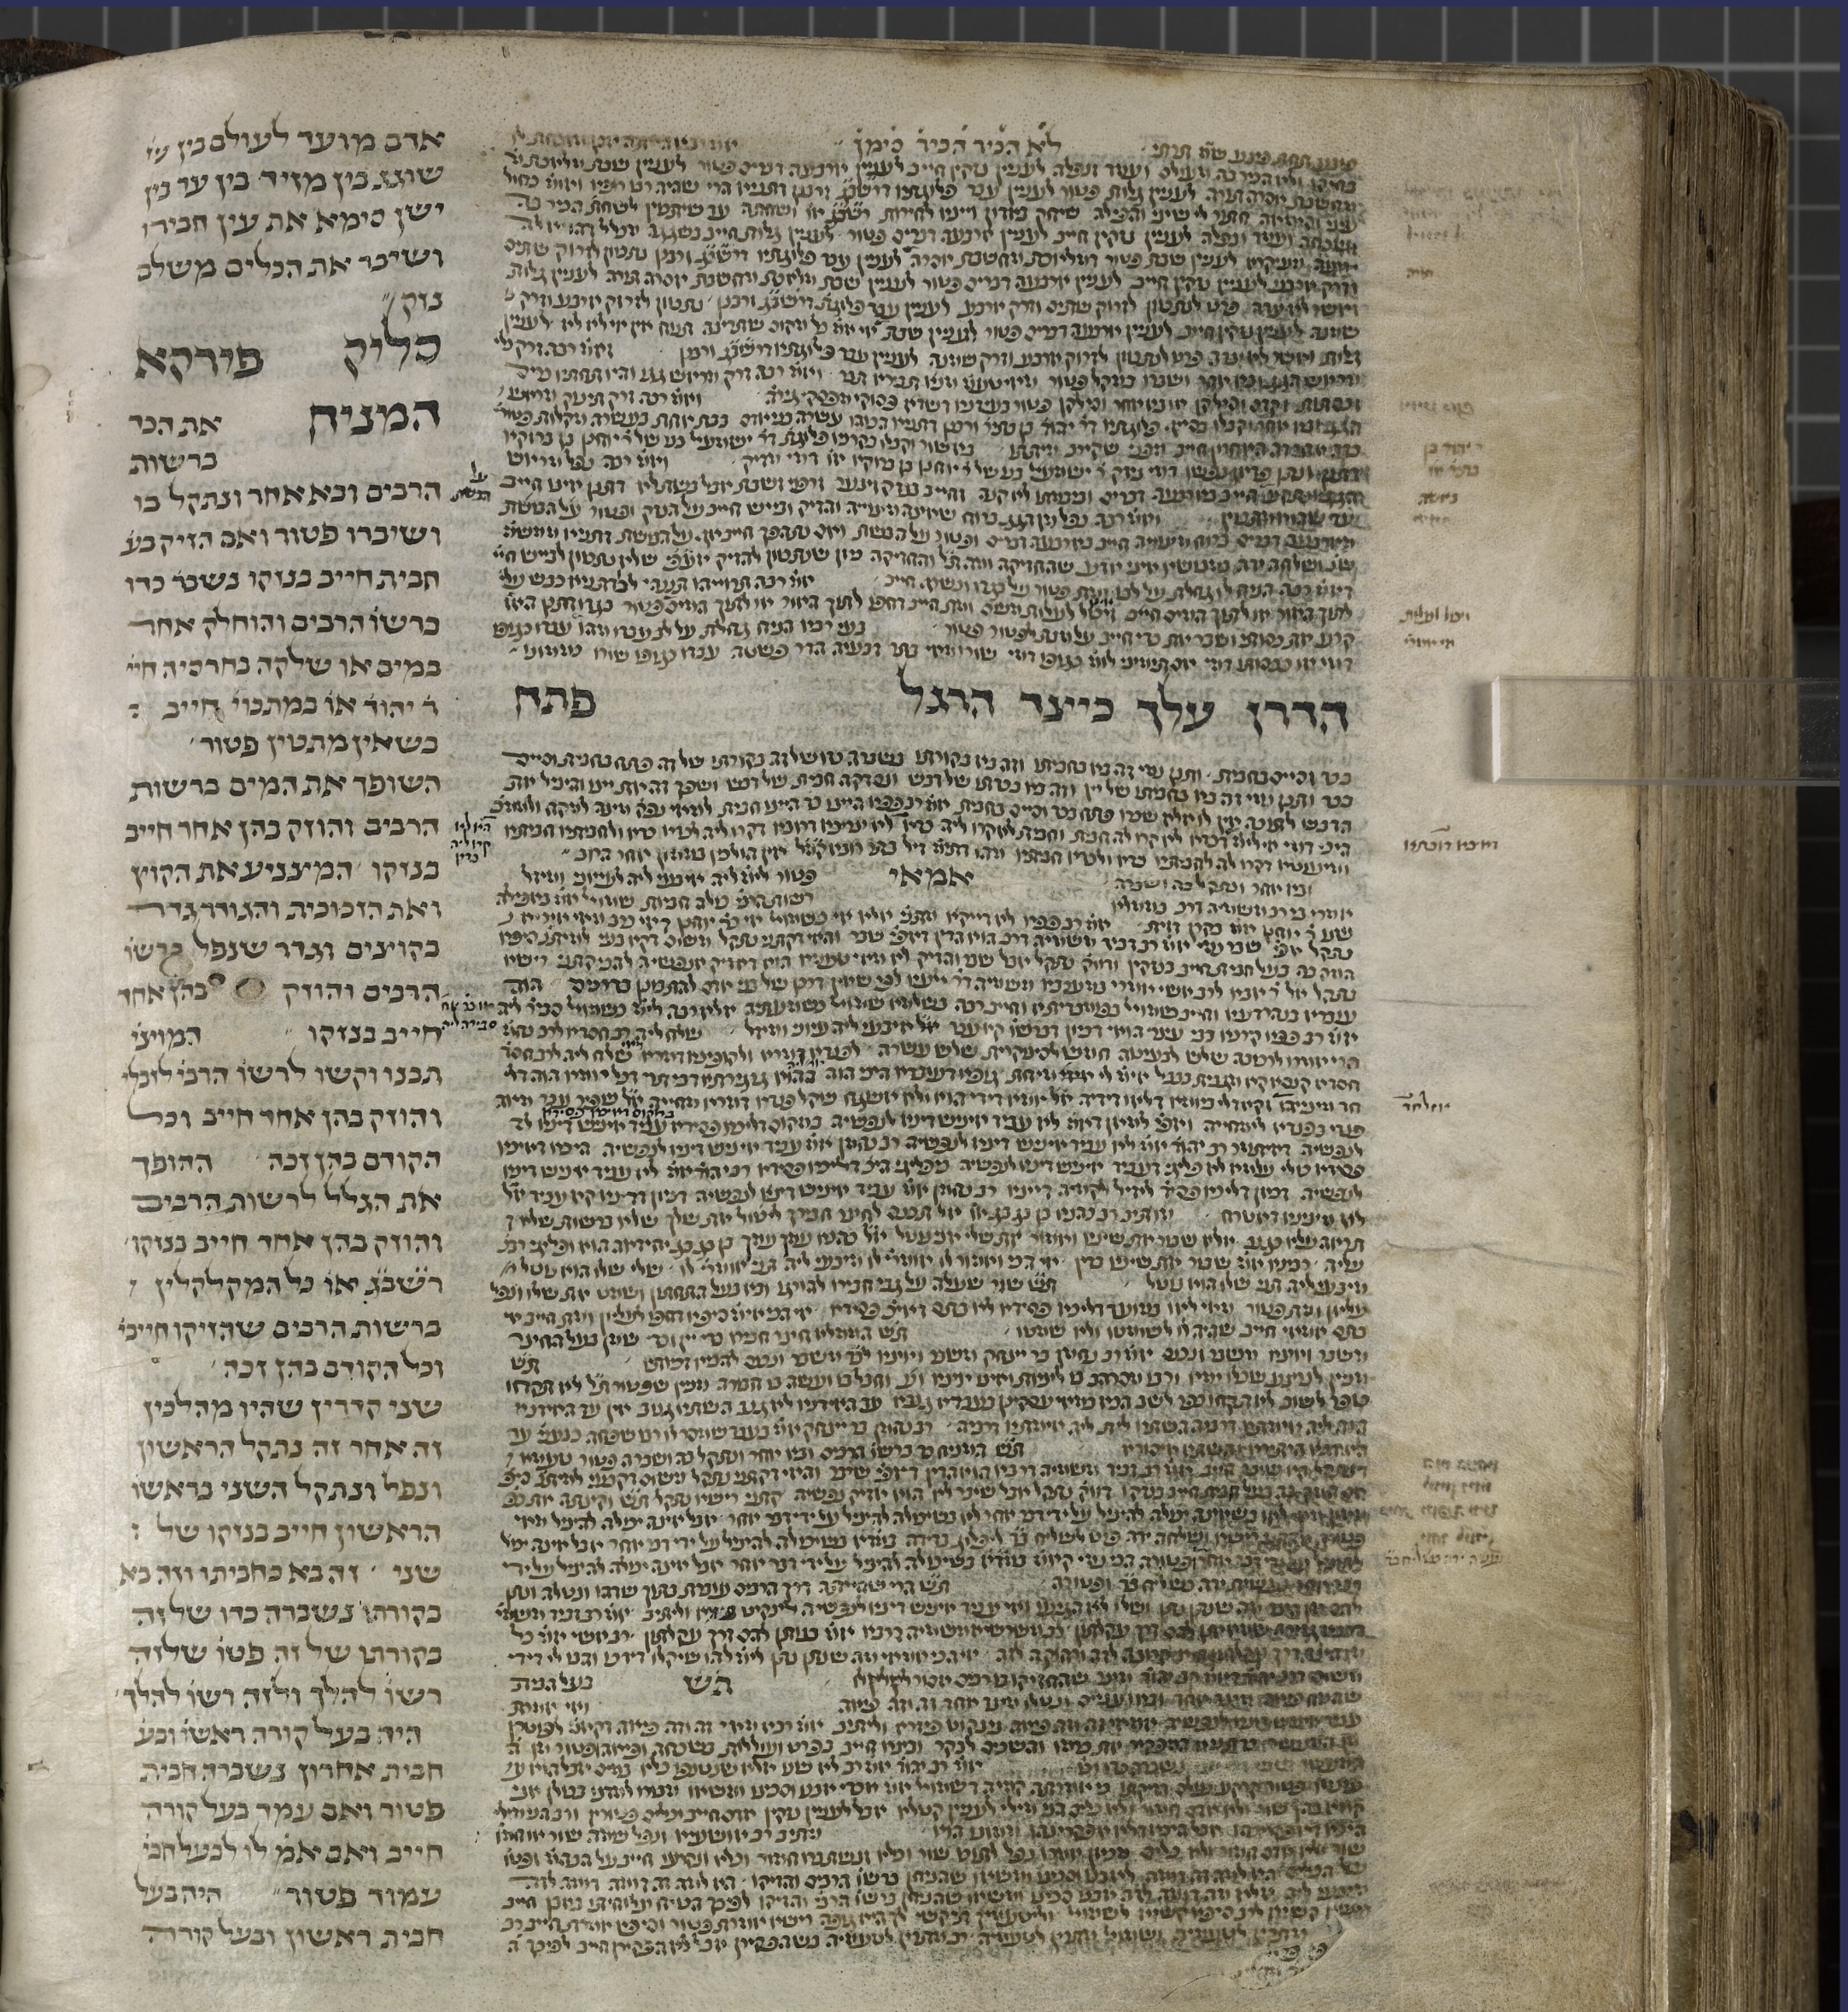
\includegraphics[trim=620 580 300 457,clip,width=0.38\linewidth]{figures/MunichTalmud.png} \\[5pt]
\raisebox{2cm}{\rotatebox{90}{Paper}} &
\includegraphics[trim=345 350 205 419,clip,width=0.38\linewidth]{figures/maimonides.jpg} &
\includegraphics[trim=300 914 350 310,clip,width=0.38\linewidth]{figures/quill on paper.jpeg} \\
\end{tabular}
\caption{Sample patches of four medieval manuscripts in Hebrew characters. Top left: calamus on parchment; top right: quill on parchment; bottom left: calamus on paper; bottom right: quill on paper. They are written in square and semi-cursive script modes,  in Hebrew, Aramaic, and/or Judeo-Arabic.
}
\label{fig:examples}
\end{figure}

From the 11th century onward, paper becomes the standard writing support for Hebrew manuscripts in the Mediterranean, and later in North Africa and Spain.
Although, in the entire corpus of the dated medieval Hebrew manuscripts, the amounts of those written on parchment and on paper are nearly equal, for some regions and regional script types the situation is different.
There are, in fact, only 28 known, dated Oriental Hebrew manuscripts on parchment (about 8\% of all dated Oriental manuscripts), and all of them were copied before the early 14th century.
On the other hand, in Ashkenaz (Germany and Central Europe), the percentage of dated manuscripts on parchment is 82\%, and reaches 100\% in some centuries.
See the book on Hebrew codicology by Malachi Beit-Ari\'e~\cite[pp.\@ 217\,ff.]{beit_arie_malachi_2021_8849}.

Recognizing the writing support of a manuscript can in many cases, as indicated above, contribute to its accurate dating and to the determination of the place of copying.
The visual appearance and characteristics of paper and parchment (especially of the hair side) are often highly informative.
The cases when a single manuscript is written partly on paper and partly on parchment, that is, paper quires  wrapped  in parchment bifolia, are also indicative.
This practice was more pronounced in Byzantium and was never adopted in the Middle East or in Ashkenaz.

Finally, when one recognizes that some leaves of a manuscript are written on parchment and others on paper but the two are not intermixed, this suggests that it may be a collection of disparate works bound together.
Many such items are yet to be identified, so they are still often mistakenly cataloged as a single work.

Differentiation between paper and parchment can easily be  performed \textit{in situ} when one can touch the manuscript pages.
Determining the writing support by image is sometimes easy, for example when one sees hair follicles on the parchment, but sometimes the two dimensional nature of an image makes this task challenging.
This is one of the cases when an algorithm can be more efficient than a human researcher.

Calamus, a reed pen, was the principle writing instrument in the Orient.
In Europe, the quill (a trimmed flight feather of a large bird) was introduced and beginning in the 6th century gradually replaced the calamus, which led to a significant change in writing techniques.
In the Italian regional type of  medieval Hebrew script, both implements are attested.
Thus, calamus and quill are associated with different script types.
In addition, there may be subtle differences in the morphology (shape) and ductus (flow) of the script depending on the writing implement.

We have prepared datasets of images of medieval Hebrew manuscripts, labeled by writing material---whether paper or parchment---and by writing implement---whether quill or reed pen,
and have trained neural networks to classify images of manuscript pages into each of the two binary categories.
\autoref{fig:examples} displays a few manuscript patches showcasing the diversity of writing tools and substrates captured in our datasets.

\section{Related Work}

In recent years, there have been extensive efforts to analyze historical manuscripts using computational tools.
These focused primarily on script classification, dating, and the like.
Codicological features have been measured computationally or with computational aids  in~\cite{Geniza,Causo}, for example.

A thorough investigation into the physical characteristics of the writing medium helps provide a more comprehensive understanding of their provenance and historical context.
This should include identifying the main components of the support, writing, and miniature materials, and assessing the evolution of their conservation state in correlation with intrinsic and environmental factors that have impacted their physical condition and visual appeal.
The substrate and the writing tool, despite their critical role in understanding historical contexts and scribal practices across different cultural and historical contexts, have received comparatively less attention.

\subsection{Support Analysis}

Advancements in analytical techniques are continuously enhancing our understanding of the materials used for writing.
Characterizing them is essential for proper preservation and serves as important evidence for codicological studies.
For example,
X-ray fluorescence (XRF) spectroscopy has been applied in~\cite{xrf} for compositional analysis, particularly for elemental mapping of inks, pigments, parchment, and paper.
An X-ray diffraction (XRD) study on 18th--19th--century South American manuscripts incorporated XRF to analyze their composition~\cite{xrd}.
Non-invasive investigations have also been conducted using multi- and hyper-spectral imaging, Fourier transform infrared (FTIR) spectroscopy, and XRF spectroscopy to obtain crucial information on parchment manufacturing techniques and original materials~\cite{ftir1}.
Furthermore, FTIR has been specifically applied to investigate degradation in parchments of various origins~\cite{ftir2}.
In a similar vein, attenuated total reflectance FTIR, micro-Raman, and XRF spectroscopies were employed to analyze fragments of different Yemenite manuscripts on both parchment and paper~\cite{yem}.
In~\cite{inkparch},
a multispectral thresholding and energy minimization (MTEM)-based pipeline for Dead Sea scroll fragments was developed, enabling the distinction and segmentation of ink from parchment by leveraging the characteristic spectral signatures of the parchment.
A classifier based on the two-dimensional Fourier transform was proposed in~\cite{Reynolds_2023,dhali2023pattern} to capture surface-level texture characteristics for distinguishing material substrates.

\subsection{Implement Analysis}

Traditional techniques for determining the specific writing tool employed (such as quill or calamus)
rely on paleographic observations of stroke morphology, pressure variations, and ink flow characteristics.
Foundational paleographic studies, such as~\cite{Bischoff_1990}, establish links between writing implements and stroke characteristics, showing that instruments like quills and reed pens produce distinct visual characteristics.
These differences are seen in the thickness and fluidity of the strokes and stem from factors such as the design of the nib, ink retention, and the way the writer holds and presses the tool while writing.

In~\cite{srihari2002individuality}, frameworks were introduced  to extract tool-specific features such as pen pressure, writing movement, and stroke-width variability using computational feature extraction and machine-learning techniques.

\section{Datasets}

The manuscript images used in this work originate from the SfarData
\footnote{\url{https://sfardata.nli.org.il/\#/startSearch_En}} and HebrewPal
\footnote{\url{https://www.hebrewpalaeography.com}}
projects,
each of which provides images of Hebrew manuscripts from a variety of historical sources, along with substantial metadata.

SfarData is the unique database developed by the Hebrew Paleography Project.
Since 1965, a group of researchers under the direction of the late Malachi Beit-Arié conducted a pioneering effort to catalog and analyze all dated or datable medieval Hebrew manuscripts produced before 1540.
During decades of work, these manuscripts were studied \textit{in situ} in over 250 public and private collections worldwide, and meticulously described codicologically (describing the writing support) with some paleographic features (describing the script).
Since the 1990s, the handwritten data has been gradually digitized and, after a series of transformations,  SfarData today exists in the form of an online database housed by the National Library of Israel~\cite{Sfardata}.

HebrewPal is the brainchild of paleographer, Judith Olszowy-Schlanger.
Launched in 2022, it is being developed to include exemplars of Hebrew books, documents, and epigraphy from all regions of the Jewish diaspora.
Images are annotated with a wealth of paleographic data, including fine-grained features of select letters.
Traditional Hebrew paleography is being combined with the latest developments in digital technology
as part of an ERC-funded project,
"MiDRASH -- Migrations of Textual and Scribal Traditions via Large-Scale Computational Analysis of Medieval Manuscripts in Hebrew Script," a computational-humanities effort aiming to reconstruct medieval Jewish book culture~\cite{Midrash}.

Our dataset images were carefully selected by the paleographer on our team to constitute a representative sample of the diversity in writing tools and substrates, ensuring that both material properties (paper or parchment) and writing characteristics (quill or calamus) are well-represented for robust classification.
To ensure accuracy of the annotations,
we used SfarData and HebrewPal as sources of metadata for the support and implement tags, respectively.

\smallskip\noindent\textbf{n.b.} \textit{The datasets will be gladly shared upon request for non-commercial research purposes.
The source code for our implementation is publicly available on
\href{https://github.com/TAU-CH/support_and_implement_classification}{GitHub}.}

\subsection{Support Dataset}

For the substrate classification task (see \autoref{tab:substrate-data}), we curated a corpus of 1,250 manuscript images, based on material annotations extracted from SfarData and the corresponding images from Ktiv.
Black-and-white images were excluded to ensure consistency in visual characteristics.
Among these, 456 manuscripts were identified as paper and 794 as parchment.
To mitigate class imbalance, two page images were sampled from each paper manuscript and one from each parchment manuscript, resulting in 912 paper and 794 parchment page images (a total of 1,706 page images) derived from 1,250 manuscripts.

\subsection{Implement Dataset}

For the writing-tool classification task (see \autoref{tab:tool-data}), we curated a corpus based on annotations from HebrewPal and high-resolution color images obtained from Ktiv.
The dataset includes 80 manuscripts, of which 40 were written with a quill and 40 with a calamus.
One page image was sampled from each manuscript, resulting in a balanced dataset comprising 40 quill and 40 calamus page images derived from distinct manuscripts.

\begin{table}[t]
\centering
\begin{minipage}[t]{0.49\linewidth}
\centering
\begin{tabular}{lr}
\hline
Items & \multicolumn{1}{c}{Quantity} \\
\hline
Manuscripts & 1,250~~ \\
Paper & 456~~ \\
Parchment & 794~~ \\
\hline\\
\end{tabular}
\caption{Writing support dataset statistics.}
\label{tab:substrate-data}
\end{minipage}
\hfill
\begin{minipage}[t]{0.49\linewidth}
\centering
\begin{tabular}{lr}
\hline
Items & \multicolumn{1}{c}{Quantity} \\
\hline
Manuscripts & 80~~ \\
Quill/Calamus (count) &  40/40~~~\\
Patches & 720~~ \\
Lines (estimate) & 4,320~~ \\
\hline
\end{tabular}
\caption{Writing implement dataset statistics.}
\label{tab:tool-data}
\end{minipage}
\end{table}

\section{Method}
Our methodology is centered on two parallel classification pipelines to analyze medieval Hebrew manuscripts, each with an approach tailored to its specific target binary classification task.
For \textit{writing implement classification} (\texttt{quill} vs.\@ \texttt{calamus}), we employ a patch-based deep-learning model, allowing the model to focus more on localized visual details (fine-grained morphological features of the script), such as stroke thickness, curvature, and ink dispersion.
In contrast, \textit{writing support classification}  (\texttt{parchment} vs.\@ \texttt{paper}) requires a more global perspective.
The objective is to analyze the broader textural characteristics of the substrate itself, emphasizing background texture and material characteristics, which are best assessed across different areas of the page.

\subsection{Support Classification: Paper vs.{} Parchment}

For the writing support classification task, we aim to distinguish manuscript pages based on whether they were written on paper or parchment.
Given the nature of this problem, we adopted a page-level approach leveraging a convolutional neural network (CNN) to capture global surface characteristics and material textures indicative of the underlying substrate.
The entire manuscript page was used as input, allowing the model to learn from visual cues present in regions surrounding the text, such as the exposed substrate around letterforms, as well as at the page edges where material properties like texture and fiber patterns are more pronounced.
The encoder is designed to learn the subtle material signals that differentiate parchment from paper, focusing on variations that may be challenging for human observers without physical examination.

We employed an EfficientNet-based architecture~\cite{EfficentNet} pretrained on ImageNet, which we fine-tuned for binary classification of paper versus parchment.
EfficientNet was chosen for its compound scaling strategy, which balances depth, width, and resolution, making it well-suited to capture fine-grained distinctions in manuscript images while maintaining computational efficiency.
The images were resized to a consistent resolution, selected to retain the visual granularity of substrate textures critical for classification, and normalized pixel intensity values to standardize input distributions across the dataset.
The resulting classifier is able to capture differences that are difficult for human experts to replicate manually at scale, providing a scalable and generalizable approach for automated material identification across a wide range of manuscripts.

\subsection{Implement Classification: Quill vs.{} Calamus}

To automatically differentiate between  a manuscript  written using a quill or with a calamus, we adapted a deep learning framework to this specific task.
The core backbone of the method is a CNN that learns to distinguish the subtle visual features associated with each tool.
High-resolution manuscript images were preprocessed, with each page being divided into smaller, non-overlapping patches of 350$\times$350 pixels.
This expands the dataset by several orders of magnitude while preserving meaningful visual features.

Paleographic studies suggest that patches containing around five lines of text are adequate for identifying the script type. Accordingly, the patch generation process ensured consistent text scale and inclusion of sufficient text lines~\cite{patch}. To ensure that only informative and content-rich patches are retained, each candidate patch undergoes a filtering step based on pixel intensity statistics:
(i) Patches with too much white space or low variation

(ii) A statistical threshold is applied using heuristics like entropy or pixel mean/variance to detect and remove low-texture regions.
This significantly improves the signal-to-noise ratio in the dataset, ensuring that models train only on visually meaningful data.

For the CNN architecture, we fine-tuned a ResNet18~\cite{resnet} model pretrained on ImageNet, applying standard image transformations (resizing, normalization).
Notably, standard data augmentation techniques such as random rotations or flips were deliberately avoided to preserve the original orientation and directionality of the script's strokes, which are crucial features for distinguishing between the flexible marks of a quill and the more rigid, angular lines of a calamus.

To mitigate the potential risk of overfitting, we employed several strategies at both the data and training levels. First, we used a patch-based approach to expand our dataset to 720 distinct image samples, providing the model with more varied examples. Second, we enforced a strict manuscript-level split, ensuring no manuscript overlap between the training and test sets. This validation strategy ensures the model's ability to generalize to entirely unseen manuscripts, rather than just new sections of familiar ones. Finally, during training, we further regularized the model using early stopping and weight decay.

\section{Results}

We evaluate the performance of our approaches using standard classification metrics including accuracy, precision, recall, and $F_1$-score, providing a comprehensive assessment of model effectiveness.

\begin{table}[t]

\centering
\begin{tabular}{lcccc}
\hline
Class & Precision & Recall & $F_1$-score & Quantity \\
\hline
Paper & 0.96 & 0.87 & 0.91 & 136 \\
Parchment & 0.86 & 0.96 & 0.91 & 120 \\
\hline
\multicolumn{5}{l}{Total accuracy = 91\%}
\end{tabular}
\caption{Writing support classification metrics.}\label{tab:3a}

\end{table}
\begin{table}[t]

\centering
\begin{tabular}{lcc}
\hline
& \multicolumn{2}{c}{Predicted} \\
Actual & Paper & Parchment \\
\hline
Paper & 118 & \phantom{1}18 \\
Parchment & \phantom{11}5 & 115 \\
\hline
\end{tabular}
\caption{Writing support confusion matrix.}\label{tab:3b}

\end{table}

\subsection{Support Classification}

Paleographers are not trained to determine the type of writing support solely from an image of a manuscript page.
As with other codicological tasks, it is performed physically, by touching and turning (and smelling) the pages of a codex.
This makes it hard to evaluate  algorithm results compared to human performance.

For most types of writing support, especially for parchment with noticeable signs on the hair side or for paper with visible texture, an image suffices to differentiate between them.
However, Ashkenazi manuscripts since the end of the 13th century (that is, in most cases, manuscripts produced in Germany---because of the 14th century expulsions of the Jews from France)  were written on parchment processed in such a way that the hair side and the flesh side became virtually indistinguishable.
In such cases, as well as in the numerous cases of very fine smooth paper with almost no signs of texture, differentiating between writing supports by image only, and without the use of paleographic features, is problematic.
For this reason and for this specific task, we believe that the algorithm is at least as effective as---and probably superior to---a flesh-and-blood scholar.

Our EfficientNet-based support classifier achieved a total accuracy of 91\%, demonstrating strong performance even on challenging manuscript images where visual cues distinguishing paper and parchment are subtle.

\autoref{tab:3a} reports aggregate classification metrics, while \autoref{tab:3b} presents the confusion matrix summarizing correct and incorrect predictions at the page level.

\subsection{Implement Classification}

At the patch level, the ResNet18-based writing-implement classifier achieved strong performance with an accuracy of 88.5\%, precision of 88.6\%, and $F_1$-score of 87.1\%.
To obtain page-level predictions, patch-wise outputs were aggregated using a majority voting strategy, yielding an accuracy of 91.5\%, precision of 93.5\%, and $F_1$-score of 90.9\%.
These results, summarized in \autoref{fig:metrics}, demonstrate that local visual cues effectively contribute to writing implement attribution, while aggregation improves robustness significantly at the page level.

To interpret the model's predictions, we visualize the most salient features using Grad-CAM~\cite{gradcam}, generating localization maps that highlight the regions of the manuscript images that were responsible for the models' decisions.
See \autoref{fig:gradcam}.
These visualizations confirm that the models are indeed focusing on key stylistic cues relevant to this classification task.
However, the visualizations also hint that the model is focusing on different features that those to which a human paleographer would pay attention.

The Grad-CAM visualizations suggest that the writing-implement model pays attention primarily to stroke morphology and junctions. The highlighted regions in the heatmaps often cover relatively broad areas, so not every activation can be tied to a single discrete paleographic feature. However many of the high activation zones coincide with serifs, hairlines, and ascenders of the letter \textit{lamed} with flags. These are the regions where differences between calamus and quill become most apparent. The difference is---first and foremost---the ability of a quill to produce very thin lines that are connected to much thicker ones (shading), and special forms such as “fishtails,” hairlines, etc. This alignment suggests that the model is, at least in part, learning genuine implement-related features.

\begin{figure}[t]
\centering
\includegraphics[trim=0 0 30 110,clip,width=\linewidth] {figures/model_eval_metrics.png}
\caption{Model evaluation metrics: Patch-level (orange) and page-level (blue) performance of writing-implement classification.}
\label{fig:metrics}
\end{figure}

\begin{figure}[t]
\centering
\includegraphics[width=0.23\textwidth]{figures/gradcam_1.png}
\includegraphics[width=0.23\textwidth]{figures/gradcam_2.png}

\includegraphics[width=0.23\textwidth]{figures/gradcam_5.png}
\includegraphics[width=0.23\textwidth]{figures/gradcam_6.png}

\caption{Grad-CAM visualizations highlighting activations focused around letter forms that strongly influence writing-implement classification.}
\label{fig:gradcam}
\end{figure}

\section{Conclusion}

In this study, we developed a machine-learning framework to classify medieval Hebrew manuscripts by writing support (paper vs.\@ parchment) and writing implement (quill vs.\@ calamus).
By curating carefully annotated datasets extracted from digitized repositories (SfarData, HebrewPal, and Ktiv) and employing convolutional neural networks tailored to each task, we demonstrated strong classification performance, with accuracy exceeding 90\% for both of the tasks.
The results show that algorithmic methods can match or surpass human expertise in certain codicological tasks where tactile examination is not feasible, providing a scalable approach for large-scale manuscript analysis.

{While our models were trained exclusively on Hebrew-character manuscripts, the underlying tasks of textural and stroke-morphology analysis are not inherently script-dependent. Therefore, we believe that this approach shows promise for generalization and could be applied to manuscripts in other languages and scripts as well.}
Additional material substrates, such as papyrus, with its distinctive fibrous structure, could easily be incorporated into such a classification scheme.

This research opens pathways for combining material analysis with script and content analysis, ultimately contributing to a deeper and more systematic understanding of medieval manuscript production across cultures.

\begin{comment}
Tables and figures should \textit{not} appear at the top of the first page above the paper title and abstract, but can be placed within the main text, as exemplified by Table~\ref{tab:example}. They may also be placed at the top of non-first pages, as exemplified by \autoref{fig:examples}.
Figures and tables discussed in the main text should appear \textit{before} the References section. Supplementary materials should be referenced by their relevant Appendix section, such as Appendix~\ref{appdx:first}.
Do \textit{not} change the font size of table and figure captions, or the spacing between text lines, section/subsection titles, tables, figures, and captions. You should size your figures and tables so that they stay within the \texttt{linewidth} of the paper.
\end{comment}

\section*{Acknowledgments}
We are grateful to the HebrewPal team for their contribution to the construction of the dataset. We would also like to thank the reviewers for their valuable comments and suggestions, which helped improve the quality of this paper.

This research was funded by
the European Union (ERC, MiDRASH, Project No.\@ 101071829.
Principal investigators: Nachum Dershowitz, Tel Aviv
University; Judith Olszowy-Schlanger, EPHE-PSL;
Avi Shmidman, Bar-Ilan University, and Daniel
Stökl Ben Ezra, EPHE-PSL).
Views and opinions
expressed are, however, those of the authors only and do not necessarily reflect those of the
European Union or the European Research Council Executive Agency. Neither the European
Union nor the granting authority can be held responsible for them.

\printbibliography

\end{document}